\documentclass[11pt,a4paper]{article}
\usepackage[left=15mm,right=15mm,top=25mm,bottom=18mm,headsep=8mm]{geometry}
\usepackage[T1]{fontenc}
\usepackage{lmodern,amsmath,amssymb,booktabs,graphicx,microtype,array,tabularx}
\usepackage[round]{natbib}
\usepackage[hidelinks]{hyperref}
\usepackage{tikz,listings,fancyhdr,longtable}
\usetikzlibrary{arrows.meta,positioning}
\setlength{\emergencystretch}{3em}
\setlength{\parskip}{4pt}
\pagestyle{fancy}\fancyhf{}
\fancyhead[L]{\small CMTF | Identification-aware expert routing}
\fancyhead[R]{\small Working paper}\fancyfoot[C]{\thepage}
\setlength{\headheight}{14pt}
\lstset{basicstyle=\ttfamily\footnotesize,breaklines=true,columns=fullflexible,keepspaces=true,showstringspaces=false,frame=single,numbers=left,numberstyle=\tiny,numbersep=5pt}
\newcommand{\systemname}{CMTF}
\title{Agentic Causal Macro Intelligence:\\An Identification-Aware Framework for\\Regime-Conditional Expert Routing}
\author{Timilehin Olapade}
\hypersetup{pdftitle={Agentic Causal Macro Intelligence: An Identification-Aware Framework for Regime-Conditional Expert Routing},pdfauthor={Timilehin Olapade},pdfsubject={Causal evidence contracts, regime uncertainty, expert routing and reproducible synthetic diagnostics},pdfkeywords={CMTF, neuro-symbolic systems, causal inference, mixture of experts, regime shift, abstention},pdflang={en}}
\begin{document}\maketitle
\begin{abstract}Regime-aware decision systems can route predictions through specialized experts, yet a well-separated latent state does not establish a valid causal mechanism. We develop the Causal Macro Transmission Framework (CMTF) as an identification-aware interface between proposed economic mechanisms, versioned evidence, and expert eligibility. A reference router checks declared identification status, provenance, numerical validity, and evidence availability before assigning normalized expert weights or abstaining. We evaluate a separate synthetic diagnostic that isolates confounding and regime-observation misspecification. Four scenarios, each with 200 independent seeds, compare pooled regressions, hard and soft filtered routing, and an oracle-state baseline over 2,000 training and 1,000 test observations. With observed confounding and a correctly specified observation model, soft routing reduces mean squared structural-coefficient error from 1.025 for pooled adjusted estimation to 0.373. Reversing the observation-to-regime mapping at test time raises soft-routing error to 2.890, above the unchanged pooled error of 1.025. With hidden confounding, even oracle-state routing retains error of approximately 1.004. These results separate state uncertainty from causal identification: improved routing cannot remove an omitted common cause, and correct local estimates can be misapplied when state semantics change. The contribution is an executable evidence contract and a reproducible failure diagnostic, not an end-to-end causal discovery system or evidence of trading profitability.\end{abstract}
\section{Introduction}
Economic narratives often specify a pathway from a macroeconomic development to an asset price. Turning such a narrative into a decision requires more than predicting a market regime. The question must specify what changes, which outcome is measured, the time horizon, the information available at the decision, and the assumptions under which the effect can be recovered from observations. A latent-state label by itself supplies none of these guarantees.

The Causal Macro Transmission Framework (CMTF) organizes this boundary between mechanism proposals and decision eligibility. It continues the author's earlier conceptual note \citep{olapade2026agentic}, while narrowing the empirical contribution to an executable routing contract and a controlled synthetic diagnostic. A neural component may propose a mechanism or forecast; a symbolic record specifies its evidence status and applicability. The implementation tested here consumes declared records. It does not use a language model to establish identification, learn an economic causal graph, or verify the truth of an assumption.

We distinguish three questions. Is a causal effect identified under a declared model? Can the execution system infer the current regime reliably? Does a proposed action match the direction, horizon, and information vintage of its supporting evidence? Failure in one cannot generally be repaired by success in another. The synthetic study isolates the first two; the router implements a minimal contract for declared evidence. Neither is presented as a full deployed neuro-symbolic trading system.

Our main finding is a reversal: filtered routing improves coefficient recovery under the nominal observation mechanism, but becomes worse than pooled adjustment after the observation-to-regime relationship is reversed. A second finding is that oracle knowledge of the regime does not remove hidden-confounding bias. Together these motivate explicit failure states rather than a single undifferentiated confidence score.

\section{Positioning and contribution}
Mixture-of-experts systems combine specialist outputs using input-dependent weights \citep{jacobs1991}. Weighting addresses which prediction to use; causal identification addresses whether the target effect is recoverable from the assumed graph and observed data. These are different operations. DoWhy explicitly separates modeling, identification, estimation, and refutation \citep{sharma2020}. CMTF adopts this separation as an interface constraint rather than introducing a replacement identification calculus.

Selective prediction permits a system to decline an output when a selection criterion is not met \citep{geifman2019selectivenet}. Our router's abstention is a deterministic contract outcome when no record passes the declared checks. It does not learn a calibrated risk/coverage trade-off. Here coverage means the fraction of cases receiving an output, and risk means the error on those retained cases; neither is measured on a real decision dataset in this study.

The original macro-to-asset framing supplies a use case, not evidence that a particular economic graph is correct. The present contribution comprises a precise record-to-routing interface, executable contract checks, and a four-scenario diagnostic with a known data-generating process. Standard regression and filtering are used to expose failure modes, not claimed as new estimators.

\section{Evidence records and routing}
\subsection{A declared causal question}
Let $X$ be a treatment variable, $Y$ an outcome, and $C$ a set of pre-treatment context variables. A treatment is the variable whose value is hypothetically changed; a context variable is observed before that change. For values $x_1,x_0$ and context $c$, a possible query is
\begin{equation}
 \tau(c)=\mathbb{E}[Y\mid\operatorname{do}(X=x_1),C=c]
 -\mathbb{E}[Y\mid\operatorname{do}(X=x_0),C=c].
\end{equation}
The scalar $\tau$ (tau) is a defined causal contrast. $\mathbb{E}$ denotes an expected value, or average under the specified distribution. The operator $\operatorname{do}$ denotes intervention: set $X$ externally rather than merely select observations with a certain $X$. The vertical bar means conditioning. This definition does not establish that the contrast can be estimated from the available data.

An evidence record should specify the query, graph version, identification argument, estimator version, units, horizon, availability time, expiry, and unresolved assumptions. An execution-state estimate is kept distinct from the pre-treatment context used for identification. Conditioning on a variable caused by the treatment can change or bias the target; a convenient state feature must not automatically be used as a causal adjustment variable.

\subsection{The implemented contract}
The reference implementation stores, for each expert $k$, a unique identifier; direction $d_k\in\{-1,0,1\}$; score $s_k$; response $r_k$; nonnegative penalty $p_k$; availability and expiry times; a declared identification flag; and a provenance string. Scores, responses, and penalties are finite scalar inputs. They are assumed to be on a compatible dimensionless scale in this demonstration. Real effects with different units or horizons require explicit conversion before aggregation.

At decision time $t$, the router rejects nonfinite values, invalid directions, negative penalties, missing provenance, records declared unidentified, and records unavailable or expired at $t$. A duplicate expert identifier raises an error. The identification flag is supplied by the caller; checking it does not prove identification. The richer graph, units, horizon, and diagnostic checks described above are an interface specification, not fully implemented validators.

For eligible expert set $\mathcal{K}_t$, the chosen logit and normalized weight are
\begin{align}
 \ell_k&=s_k+d_kr_k-p_k,\\
 w_k&=\frac{\exp(\ell_k-m)}{\sum_{j\in\mathcal{K}_t}\exp(\ell_j-m)},\qquad
 m=\max_{j\in\mathcal{K}_t}\ell_j.
\end{align}
Here $\ell$ (ell) is a scalar routing score, $w_k$ is a nonnegative weight, $\exp$ is the exponential function, and $j$ indexes eligible experts. The set $\mathcal{K}_t$ contains only records that passed the contract. Subtracting the maximum $m$ leaves the normalized ratios unchanged while preventing exponential overflow. The weights sum to one. If the eligible set is empty, the output is an abstention record with reasons; the denominator is never evaluated.

The direction term rewards alignment with the signed response. For example, with score 0.2, response $-0.8$, and penalty 0.1, a long proposal has logit $0.2-0.8-0.1=-0.7$, while a short proposal has logit $0.2+0.8-0.1=0.9$. With only these two eligible experts, their weights are approximately 0.168 and 0.832. A future-dated proposal is rejected even if its numerical score is very large. The example explains contract behavior; these numbers are not calibrated trading preferences.

The algorithm scans records once for validation, computes eligible logits, and normalizes them. A dictionary stores rejection reasons keyed by expert identifier, and another stores eligible weights. For $K$ records, both time and storage grow linearly, written $O(K)$: doubling the number of records approximately doubles the work and retained entries. Portfolio constraints and order execution occur after routing and are outside this demonstration.

\section{Synthetic diagnostic}
\subsection{Data-generating process}
Each dataset contains 3,000 sequential observations: 2,000 training and 1,000 test. Let $S_t\in\{0,1\}$ be a latent regime with transition matrix
\begin{equation}
 A=\begin{pmatrix}0.97&0.03\\0.03&0.97\end{pmatrix}.
\end{equation}
$A$ is a chosen $2\times2$ matrix: row $j$ gives the probabilities of the next regime conditional on current regime $j$. It encodes persistence, not a fitted market model. The initial regime is sampled uniformly. Independent standard-normal random variables $C_t,U_t,V_t,W_t$ generate
\begin{align}
 X_t&=C_t+U_t,\\
 Y_t&=\theta_{S_t}X_t+2C_t+V_t,\\
 M_t&=\mu_{S_t}+\sigma_M W_t.
\end{align}
The scalar $C_t$ is a common cause of treatment $X_t$ and outcome $Y_t$; $U_t$ and $V_t$ are independent disturbances. $M_t$ is a noisy regime observation, not an outcome or treatment. The chosen coefficient vector $\theta$ (theta) is $(1,-1)$ except in the inactive-second-regime scenario, where it is $(1,0)$. The chosen emission-mean vector $\mu$ (mu) is $(-0.7,0.7)$, and $\sigma_M=1.3$ (sigma) is observation noise standard deviation. Each vector has two entries, one per regime. All observations are synthetic and use arbitrary units.

The four scenarios are observed confounding, hidden confounding, test-time emission reversal, and an inactive second regime. In the hidden-confounder case $C_t$ exists but is unavailable to the estimators. In emission reversal, test observations use $-\mu_{S_t}$ while the filter retains nominal means. Structural coefficients do not change. This isolates a change in how the regime is observed from a change in the underlying outcome mechanism.

\subsection{Estimation and filtering}
The training regime labels are supplied as oracle information, meaning the simulator's true states are revealed to the estimator. We estimate a slope $\widehat\beta_k$ separately within each training state $k$. With observed confounding, ordinary least squares regresses $Y$ on an intercept, $X$, and $C$; otherwise it uses an intercept and $X$. The hat denotes an estimate. Pooled baselines fit the analogous regression without splitting by state.

The filter receives only the sequential observations $M_t$ and the fixed nominal transition and emission parameters. Let $q_{t,k}$ be its posterior probability of state $k$. Prediction and observation updating are
\begin{align}
 \widetilde q_{t,k}&=\sum_{j=0}^1q_{t-1,j}A_{jk},\\
 q_{t,k}&=\frac{\widetilde q_{t,k}L_k(M_t)}{\sum_{j=0}^1\widetilde q_{t,j}L_j(M_t)}.
\end{align}
$\widetilde q$ is the predicted probability before seeing the current observation; $L_k$ is the normal observation likelihood in state $k$. The first step uses prior $(0.5,0.5)$. Multiplication by likelihood favors states whose observation model better explains $M_t$, then division makes probabilities sum to one. Filtering runs over the training and test observation sequence, without access to test $X,Y,C$, or true $S$.

Hard routing selects the slope of the most probable state. Soft routing averages the two slopes using posterior probabilities. Oracle routing selects the slope of the true test state:
\begin{align}
 \widehat\theta^{\rm hard}_t&=\widehat\beta_{\arg\max_k q_{t,k}},\\
 \widehat\theta^{\rm soft}_t&=\sum_{k=0}^1q_{t,k}\widehat\beta_k,\qquad
 \widehat\theta^{\rm oracle}_t=\widehat\beta_{S_t}.
\end{align}
$\arg\max$ returns the state index with the largest probability. Superscripts name methods, not powers. These estimated scalars target the structural coefficient at each test time, rather than the realized outcome $Y_t$.

For test length $T=1{,}000$, coefficient mean squared error is
\begin{equation}
 \mathrm{MSE}=T^{-1}\sum_{t\in\mathrm{test}}
 (\widehat\theta_t-\theta_{S_t})^2.
\end{equation}
MSE averages squared coefficient-estimation errors; lower is better. It is not price-forecast loss or portfolio return. We use 200 independent seed values, $20260906+r$ for replicate index $r=0,\ldots,199$, reusing seeds across scenarios and methods for paired comparisons. Four scenarios times 200 datasets times five methods produce 4,000 method-level result rows, not 4,000 independent datasets.

\section{Results}
\begin{table*}[t]
\centering
\caption{Mean structural-coefficient MSE with Monte Carlo standard error in parentheses, across 200 independent datasets per scenario. These uncertainty measures describe simulation replication, not confidence in a real economic mechanism.}
\small
\setlength{\tabcolsep}{3pt}
\begin{tabular}{lrrrr}\toprule
Method & Observed confounder & Hidden confounder & Emission reversal & Inactive regime\\\midrule
Pooled unadjusted & 2.048 (.0358) & 2.048 (.0358) & 2.048 (.0358) & 1.270 (.0180)\\
Pooled available adjustment & 1.025 (.0047) & 2.048 (.0358) & 1.025 (.0047) & .257 (.0013)\\
Filtered hard routing & .503 (.0066) & 1.497 (.0098) & 3.501 (.0095) & .126 (.0017)\\
Filtered soft routing & .373 (.0041) & 1.365 (.0097) & 2.890 (.0084) & .094 (.0010)\\
Oracle-state routing & .001 (.0001) & 1.004 (.0040) & .001 (.0001) & .001 (.0001)\\\bottomrule
\end{tabular}\label{tab:cmtf}
\end{table*}

With observed confounding and the nominal observation mechanism, soft routing reduces mean MSE from 1.024985 for pooled adjustment to 0.373368. The reduction is 63.6\% relative to that particular baseline, calculated as one minus the ratio of the two mean errors. Hard routing has error 0.503279. The paired hard-minus-soft difference is 0.129911 with Monte Carlo standard error 0.002849. Soft routing benefits from representing uncertainty rather than making a discrete state choice.

The ranking also depends on the loss function. In the nominal setting, mean absolute coefficient error is 0.374484 for soft routing and 0.272642 for hard routing, so the squared-error advantage is not a universal accuracy advantage. Absolute error averages the magnitude of deviations without squaring them.

The benefit is conditional. Under emission reversal, soft-routing MSE is 2.890335 and hard-routing MSE is 3.500872, both worse than pooled adjustment at 1.024985. Oracle-state error remains approximately 0.000968 because structural coefficients and the training estimates are unchanged. The failure therefore arises from applying otherwise useful local estimates through an incorrect observation-to-mechanism mapping.

With hidden confounding, oracle-state routing has error 1.003865. Correct state selection cannot remove omitted-variable bias. Soft routing improves on the pooled unadjusted baseline but still has error 1.365132; a relative gain must not be mistaken for identification. In the inactive-second-regime case, soft-routing error is 0.093935 versus 0.256786 for pooled adjustment. The outcome metric remains coefficient error: no economic value of abstention or inactivity is inferred.

\begin{figure}[t]
\centering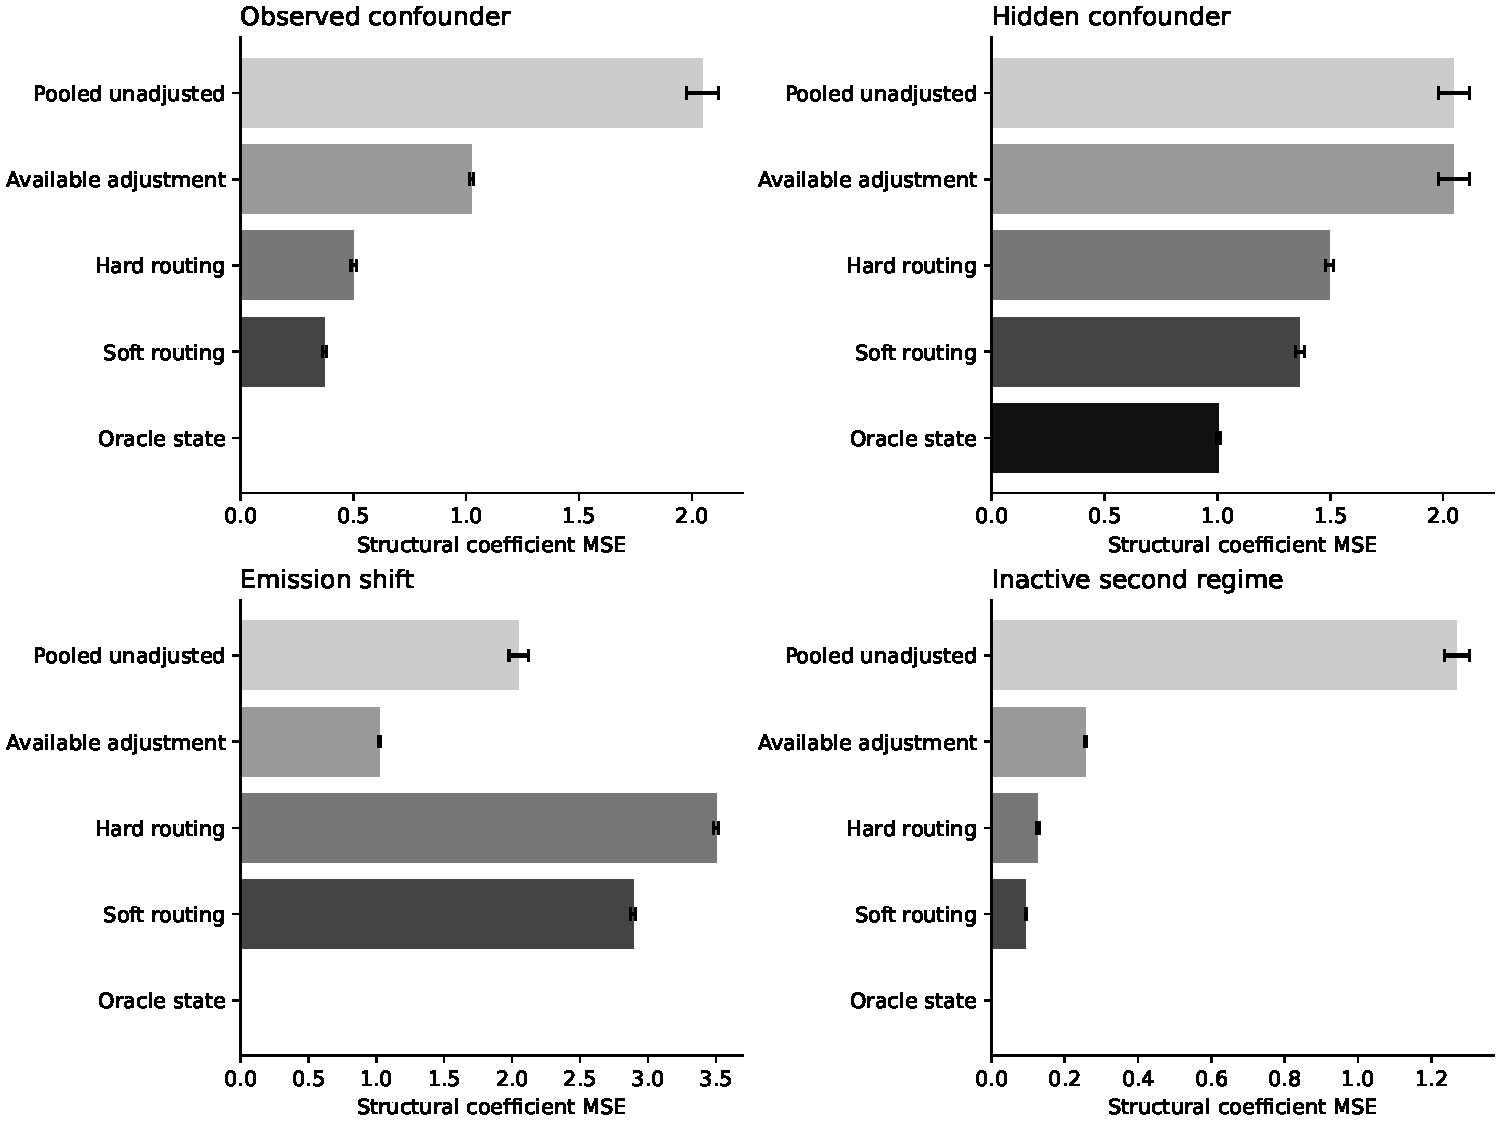
\includegraphics[width=\linewidth]{assets/synthetic_results.pdf}
\caption{Routing performance depends on both confounding and the validity of the regime observation model. Error bars are 1.96 times the Monte Carlo standard error of mean MSE.}
\end{figure}

\section{Understanding the failure mechanisms}
\subsection{Why oracle regimes do not repair confounding}
Within either regime, $X=C+U$ and $Y=\theta_k X+2C+V$. Independent standard-normal $C,U,V$ give $\operatorname{Var}(X)=2$ and $\operatorname{Cov}(X,C)=1$. Variance measures spread and covariance measures joint variation. The population unadjusted regression slope is therefore
\begin{align}
 \beta_k^{\rm unadjusted}
 &=\frac{\operatorname{Cov}(X,Y\mid S=k)}{\operatorname{Var}(X\mid S=k)}\\
 &=\theta_k+2\frac{\operatorname{Cov}(X,C)}{\operatorname{Var}(X)}
 =\theta_k+1.
\end{align}
We first substitute the outcome equation into covariance, then use independence to remove covariance with $V$, and finally substitute the known variances. The coefficient bias is one, giving squared error one even with perfect state selection and unlimited training data. Finite-sample estimation explains the small departure of the simulated mean from one. This is a property of the declared synthetic model, not a theorem about all hidden-confounder settings.

\subsection{Why probability weighting can help and still fail}
Suppose for this explanation that the state coefficients are known exactly and the filter probabilities are correct. Let $B=\theta_{S_t}$ be the unknown coefficient and $\mathcal{I}_t$ the information available to the filter. For any proposed scalar estimate $a$, write $\bar b=\mathbb{E}[B\mid\mathcal{I}_t]$. Expanding the square gives
\begin{align}
 \mathbb{E}[(B-a)^2\mid\mathcal{I}_t]
 =\operatorname{Var}(B\mid\mathcal{I}_t)+(\bar b-a)^2.
\end{align}
The cross term vanishes because $B-\bar b$ has conditional mean zero. The first term does not depend on $a$, so choosing $a=\bar b=\sum_kq_{t,k}\theta_k$ minimizes conditional squared error. This familiar conditional-mean identity explains soft weighting under its assumptions; estimated coefficients and a misspecified filter need not attain that optimum.

For example, with state coefficients $(1,-1)$ and probabilities $(0.6,0.4)$, soft weighting gives $0.2$. Its conditional MSE is $0.6(1-0.2)^2+0.4(-1-0.2)^2=0.96$. Hard selection gives 1 and MSE $0.4(-1-1)^2=1.6$. If the true coefficient is 1 but a reversed observation model assigns probabilities $(0.1,0.9)$, soft weighting gives $-0.8$ and squared error 3.24. A pooled coefficient near zero then has error near one. Reduced decisiveness helps under uncertainty; incorrect state semantics can dominate that benefit.

\section{Reproducibility and limitations}
All diagnostic data are generated from declared random seeds; no proprietary market data, model API, or accelerator is required. The artifact contains the generator, regressions, filter, router, tests, raw replicate results, and aggregation instructions. Regression design matrices have either two columns (intercept and treatment) or three (also confounder). Each row is one training observation. With this fixed small column count, least-squares work grows approximately linearly with training length. Filtering two states also takes linear time and stores a two-column probability array over the sequence. The reference router passes five contract tests; these tests exercise declared behavior rather than proving economic assumptions.

Training states and nominal filter parameters are oracle inputs. Results therefore isolate specified failure modes and do not establish performance with learned regimes. The evidence router and statistical diagnostic are separate modules: the routing weights from evidence scores are not the filter probabilities used in Table~\ref{tab:cmtf}. No end-to-end experiment combines language-model proposals, graph identification, estimation, regime learning, and trade execution.

The synthetic graph is deliberately simple, with a known treatment effect and independent disturbances. Real economic mechanisms may involve simultaneous feedback, unobserved interventions, revised data vintages, weak support, and multiple plausible graphs. Confidence in a predicted regime is not a calibrated probability that a causal assumption is true. The declaration of identification can itself be wrong; the current router cannot discover that fact.


\section{Architectural implications and evaluation boundaries}
\subsection{From a macroeconomic proposal to an inspectable decision}
A concrete use case is a proposal that an unexpected policy-rate increase changes an asset price through interest-rate expectations and financing conditions. The neural component can extract a candidate event and suggest a pathway. CMTF then requires an explicit question: which surprise measure, which asset outcome, which horizon, and which information vintage? An announcement can reveal economic information as well as change policy. Consequently, calling it a policy shock does not make the treatment independent of other causes of the outcome.

Identification means that the target causal effect is determined by the assumed model and the distribution of observed variables. Estimation means calculating a numerical approximation from a finite sample after choosing an identification argument. Neither a plausible narrative nor a high regime probability substitutes for that argument. An evidence contract is the structured record that keeps these distinctions attached to a proposal as it passes between components.

\begin{figure}[htbp]
\centering
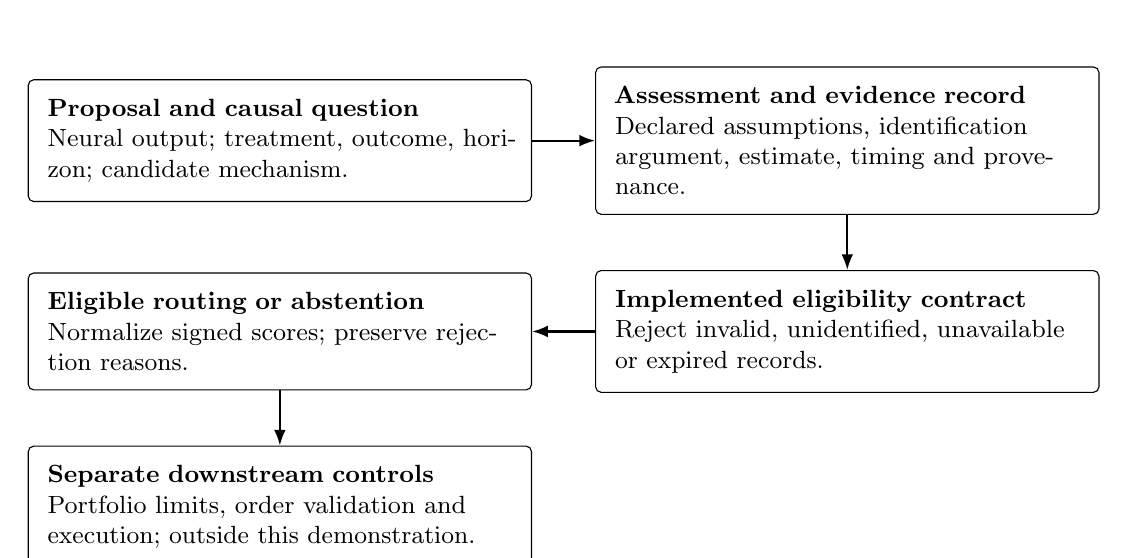
\begin{tikzpicture}[node distance=7mm and 8mm,box/.style={draw,rounded corners=2pt,text width=5.9cm,align=left,inner sep=7pt,font=\small},arr/.style={-{Latex[length=2mm]},thick}]
\node[box] (p) {\textbf{Proposal and causal question}\\Neural output; treatment, outcome, horizon; candidate mechanism.};
\node[box,right=of p] (a) {\textbf{Assessment and evidence record}\\Declared assumptions, identification argument, estimate, timing and provenance.};
\node[box,below=of a] (g) {\textbf{Implemented eligibility contract}\\Reject invalid, unidentified, unavailable or expired records.};
\node[box,left=of g] (r) {\textbf{Eligible routing or abstention}\\Normalize signed scores; preserve rejection reasons.};
\node[box,below=of r] (x) {\textbf{Separate downstream controls}\\Portfolio limits, order validation and execution; outside this demonstration.};
\draw[arr] (p)--(a);\draw[arr] (a)--(g);\draw[arr] (g)--(r);\draw[arr] (r)--(x);
\end{tikzpicture}
\caption{The proposed architecture separates semantic assessment from mechanical eligibility checks. Only the eligibility and routing contract is implemented here. Neural generation, economic identification and execution are not validated by this diagram. The synthetic regime filter is a separate diagnostic module.}
\end{figure}

\subsection{What the current gate guarantees}
For correctly typed inputs, the implemented contract ensures that every weighted record passed the listed checks at the supplied decision time. It does not ensure that the supplied time is correct, that a provenance string points to a genuine source, or that a declared identification argument is true. Timestamps in the reference example are integer clock values; a production interface must reconcile time zones, publication times, revisions and clock synchronization before passing them to the gate. The availability interval includes both endpoints.

Eligibility is therefore a necessary interface condition, not a sufficient economic guarantee. A false identification declaration can pass. An accurate estimate can be ineligible because it was unavailable at the decision time. A correctly rejected proposal can leave a profitable opportunity unused. These possibilities are features of the distinction between evidence discipline and investment performance, rather than contradictions.

\subsection{An elementary normalization guarantee}
For a nonempty finite eligible set, the largest logit $m$ exists. Every difference $\ell_k-m$ is nonpositive, so its exponential lies between zero and one in floating-point computation; at least one equals one. The sum in the denominator is therefore positive. Dividing each exponential by that common sum produces nonnegative weights summing to one, up to rounding. In exact arithmetic all weights are positive; extremely small terms can underflow to zero in floating point. Subtracting $m$ is valid because multiplying every original exponential by the same positive factor $\exp(-m)$ cancels between numerator and denominator. This is a numerical guarantee about normalization, not a calibration claim about confidence.

\subsection{Adaptation, alpha decay and hardware}
Alpha decay denotes deterioration of a strategy's risk-adjusted excess return after costs. A stale causal explanation or an obsolete observation-to-regime mapping is one possible source of deterioration. Evidence expiry, provenance checks and explicit rejection reasons can make such failures easier to inspect. The experiment does not measure alpha, detect its decay, or establish that this architecture combats it in live markets. The adverse emission-shift result instead shows why a regime-conditioned architecture requires monitoring of state meaning as well as state confidence.

An evaluation of actual adaptability would need chronological data, realistic execution costs, independent test periods, learned regimes, matched risk budgets and comparisons against simpler abstention rules. A causal gate should be compared with a gate that merely reduces exposure; otherwise lower losses may reflect less trading rather than better causal reasoning. These are prospective requirements, not completed experiments.

An FPGA (field-programmable gate array: reconfigurable digital hardware) could execute bounded comparisons, validity flags and routing arithmetic. A proposed partition would leave graph assessment and evidence construction on a host processor and pass bounded records to hardware for eligibility and normalization. Fixed-point arithmetic represents numbers with a fixed scale and finite range; it would require explicit overflow, underflow and approximation tests against the floating-point reference. No hardware implementation, latency measurement, energy benchmark or acceleration factor is reported. Hardware cannot make an unsupported identification declaration true.

\section{Conclusion}
CMTF makes the boundary between a proposed mechanism and an eligible decision explicit. Its implemented contribution is a small, inspectable contract for declared evidence; its empirical contribution is a reproducible diagnostic showing how confounding and regime-observation error affect coefficient routing. Under a valid observation model, soft routing improves coefficient recovery. Under hidden confounding, even oracle routing remains biased. Under reversed state semantics, filtered routing becomes worse than pooled adjustment. These outcomes support explicit identification status, provenance, and failure handling, while leaving live economic effectiveness and full neuro-symbolic integration open to separate evaluation.



\section*{Data, code, and scope}
The synthetic study and public aggregate results accompany this paper. No provider keys, private trading logs, account identifiers, or original model prompts are included in the public release. The public code does not execute trades or invoke paid model services. Operational results, where discussed, are descriptive source audits with restricted raw-data availability. This paper does not report investment advice, verified risk-adjusted profitability, or a causal effect in an actual market.

\bibliographystyle{plainnat}\bibliography{references}
\clearpage\appendix\section{Algorithm and code mapping}
In \texttt{synthetic\_study.py}, \texttt{state} stores the integer regime sequence, \texttt{c/x/y/m} store the common cause, treatment, outcome, and regime observation, and \texttt{q} stores a matrix with one row per time and two state-probability columns. \texttt{A}, \texttt{MEANS}, and \texttt{SIGMA} implement the transition matrix, emission means, and observation standard deviation. \texttt{beta} is the two-element vector of fitted state-specific slopes. Matrix multiplication \texttt{q @ beta} takes the probability-weighted sum for each row and returns a vector of coefficient predictions.

The generator first samples a state sequence, then independent disturbances, then constructs treatment, outcome, and observation arrays. The filter processes observations sequentially. Regression uses only the training segment and oracle training states. Predictions are evaluated on test coefficients supplied by the simulator. This ordering isolates observation-model failure and avoids fitting regression coefficients on test outcomes.

The router processes a list of immutable evidence records. It first checks unique identifiers, then records a reason for each rejected item. Valid logits enter a stable exponential normalization. An empty eligible list returns abstention. The output dictionary contains status, weights, and rejection reasons. It contains no broker order and does not execute any action.

\section{Paired differences and numerical scope}
The mean hard-minus-soft MSE differences are 0.129911 (Monte Carlo standard error 0.002849), 0.131984 (0.005207), 0.610536 (0.003371), and 0.032484 (0.000783) for observed confounding, hidden confounding, emission reversal, and inactive second regime, respectively. Each difference is first computed within the same replicate. Its standard deviation across 200 replicates is divided by $\sqrt{200}$ to obtain the reported standard error. This avoids treating correlated methods as independent observations.

The conditional-mean derivation in the main text assumes exact coefficients and correct posterior probabilities. The experiment uses estimated coefficients and, deliberately in one scenario, wrong emission parameters. The mathematical identity is an explanation of the nominal behavior, not a guarantee for the implemented filter under misspecification.

\section{Execution and artifact availability}
Run \texttt{python reproduce.py} at the public package root. The diagnostic outputs include raw replicate MSE and mean absolute error, summary means and standard errors, state-recovery diagnostics, paired comparisons, and an environment manifest. Mean absolute error averages the absolute rather than squared coefficient deviation and is provided as a secondary diagnostic. No raw financial or user data are required for this paper's numerical tables.

The implementation uses CPU-based NumPy and pandas; no GPU or provider endpoint is invoked. The reproduced environment uses Python 3.12.14, NumPy 2.3.5, pandas 2.2.3, and Matplotlib 3.10.8. The package pins its three runtime dependencies; SciPy and scikit-learn are not required. The seed schedule and nominal parameters are fixed in the supplied script. Five router contract tests cover implemented behavior. Full statistical results consist of 800 generated datasets and 4,000 method rows.

\section{Relationship to the companion study}
The companion market study uses an operational audit, exported directional responses, and a separate price-feedback simulator. It does not evaluate this evidence router as a live causal controller. Conversely, the present study does not reuse market returns as evidence of causal identification. The earlier deployment-audit study has distinct market outcome measures. The later manuscript entitled \emph{Market Transitions under AI Financial Models: Alpha Decay, Instability, and Evidence-Gated Neuro-Symbolic Adaptation} also incorporates this same four-scenario diagnostic and reference router. Those shared results are reused evidence, not independent replications or additional discoveries. This architecture paper develops their interface and identification interpretation; the market manuscript adds a separate feedback simulation. Any joint publication should disclose this overlap explicitly. The original conceptual note is cited as prior work rather than described as an independent evaluation.

\section{Notation and implementation guide}
\subsection{Objects, indices and operations}
The index $t$ labels an observation time; $k$ and $j$ label the two regimes or eligible experts as specified locally. A subscript selects an element, so $A_{jk}$ is the entry in row $j$, column $k$ of transition matrix $A$. The regime variable $S_t$ is an integer random variable; $X_t,Y_t,C_t,M_t$ are scalar random variables. Lowercase code arrays store their realized numerical samples. The expression $\sum$ denotes addition over the specified index. A superscript naming a method is a label, not exponentiation; the superscript 2 in squared error is multiplication of a number by itself.

The vectors $\theta$, $\mu$ and $q_t$ each contain two scalar entries. $\theta$ (theta) contains chosen structural coefficients, $\mu$ (mu) contains chosen observation means, and $q_t$ contains calculated state probabilities. $\sigma_M$ (sigma) is a chosen scalar standard deviation. $\beta$ (beta) denotes regression slopes; a hat marks an estimated quantity. $\ell$ (ell) denotes a calculated routing logit. $\tau$ (tau) denotes the defined intervention contrast. The set $\mathcal{I}_t$ denotes information available to the filter; $\mathcal{K}_t$ denotes eligible expert indices. These are different objects and must not be interchanged.

\subsection{Synthetic algorithm before code}
The problem is to recover a changing structural coefficient when both confounding and uncertainty about regimes are possible. A naive pooled regression ignores regime changes; an unadjusted regression also mixes the treatment effect with the effect of a shared cause. State-specific regression can address the first issue only when states are supplied or estimated appropriately. Adjustment can address the second issue only under the specified causal assumptions and availability of the confounder.

The reproducible algorithm therefore generates a known two-state process, creates treatment and outcome samples, fits training slopes within the supplied true states, filters noisy state observations, and evaluates coefficient recovery on held-out observations. Hard routing commits to one state; soft routing averages estimates; oracle routing uses the true test state as a diagnostic baseline. The known truth is used for evaluation, never as an input to the test filter. No neural network is trained in this synthetic experiment.

\subsection{Reading the generator and regression code}
\texttt{default\_rng} creates a random-number generator from a recorded seed. Reusing a seed reproduces the random stream within the stated numerical environment. \texttt{np.zeros(n,dtype=int)} allocates an integer array of length $n$; successive assignments update the stored regime. \texttt{A[state[t-1]]} selects the probability row for the previous state. \texttt{rng.choice} draws the next state using that row. Independent calls to \texttt{rng.normal} create disturbance arrays. Indexing \texttt{theta[state]} selects one coefficient for each stored regime and therefore returns an array with one coefficient per observation.

\texttt{NTRAIN:} means all array positions from the training boundary onward. The emission-reversal scenario creates new test observation noise after reversing the means; it does not change treatment or outcome equations. This preserves paired treatment/outcome data while changing the filter's test inputs.

\texttt{np.column\_stack} constructs a two-dimensional regression design: rows are samples, columns are intercept, treatment and optionally confounder. With $n_k$ training samples in state $k$, the design has shape $n_k\times3$ when adjusted and $n_k\times2$ otherwise. \texttt{lstsq} finds coefficients minimizing the sum of squared residuals. The first returned object is the coefficient vector; its second entry, index 1 in Python's zero-based indexing, is the treatment slope. No matrix inverse is formed explicitly.

\subsection{Reading the filter and evaluation code}
\texttt{q @ A} multiplies a length-two probability vector by a two-by-two transition matrix to predict the next state's probabilities. The likelihood calculation subtracts its largest logarithmic value before exponentiation. Since the states have the same observation standard deviation, their common normal-density factor cancels during normalization. \texttt{q /= q.sum()} updates the probability vector in place by dividing by its sum. The output array has one row per observation and two probability columns; the training rows are removed before test evaluation.

\texttt{q @ beta} multiplies a test-length-by-two matrix by a length-two vector, producing one coefficient estimate per test row. \texttt{argmax(axis=1)} chooses the largest probability's column separately in each row; ties select the first index. \texttt{np.full} fills a test vector with a pooled estimate. \texttt{theta[state[test]]} retrieves the simulator's true test coefficient for scoring only. Squared errors penalize large deviations more than absolute errors.

A list of dictionaries collects one result per scenario, replicate and method. Each dictionary maps a field name to a value. A pandas DataFrame turns these records into a table. Grouping by scenario and method produces summary means and standard deviations; the standard error of the mean is the across-replicate standard deviation divided by the square root of 200. The 1,000 temporally dependent test points within a replicate are not treated as 1,000 independent replications.

\subsection{Reading the evidence-router code}
The \texttt{@dataclass(frozen=True)} decorator defines a record with named fields and prevents ordinary reassignment after creation. Type annotations describe intended input types; they are not a comprehensive runtime schema validator. The brace expression collecting expert names creates a set, which contains each name once. Comparing its size with the input length detects duplicate names. A \texttt{ValueError} stops processing rather than silently overwriting an expert.

The router scans each record through an ordered sequence of tests. \texttt{all} requires every numeric field to be finite; \texttt{isfinite} excludes infinities and missing-number values. \texttt{elif} means a later check runs only if earlier conditions did not match, so the output reports the first rejection reason. A list stores eligible identifier--logit pairs; a dictionary maps rejected identifiers to reasons. If no record remains, the function returns abstention immediately. Otherwise it computes stable exponential weights. The final dictionary contains a status, weights and rejection reasons, and never contains a broker order.

For $K$ evidence records, validation and normalization require $O(K)$ time and storage: work and retained entries grow proportionally to the record count, assuming ordinary dictionary and set operations. With the fixed two-state model and fixed regression column count, the diagnostic cost grows approximately linearly with sequence length and the number of replicates. Storing all replicate-level outcomes uses space proportional to the number of scenario--replicate--method combinations.

\section{Complete reference evidence router}
\lstinputlisting[language=Python]{cmtf/evidence_router.py}
\section{Complete synthetic diagnostic}
\lstinputlisting[language=Python]{cmtf/synthetic_study.py}

\end{document}
